\documentclass[tikz]{standalone}

\usepackage{bm}
\usepackage{amsmath}

\usepackage{tikz} % Graph drawing
\usetikzlibrary{graphs, angles, quotes, babel, matrix, decorations.pathreplacing, calc, positioning, backgrounds} 

\tikzstyle{underbrace style}=[decorate, thick, decoration={brace,raise=1.5mm,amplitude=3pt,mirror}]
\tikzstyle{underbrace text style}=[font=\footnotesize, below, pos=.5, yshift=-2.5mm]


\begin{document}
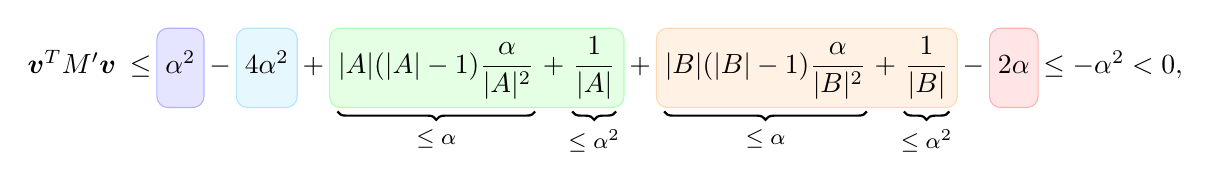
\begin{tikzpicture}            
    \matrix[name=M1, matrix of math nodes, inner sep=0pt, column sep=5pt]{
        \node (schema) [text=black] {\bm{v}^T M' \bm{v}}; & 
        \node (schema-spezifisch) [text=black] {\le}; & 
        \node (x) [text=black] {\alpha^2}; &
        \node (y) [text=black] {-}; & 
        \node (a) [text=black] {4\alpha^2}; &
        \node (b) [text=black] {+}; &
        \node (c) [text=black] { |A|( |A| - 1) {\dfrac{\alpha}{|A|^2} }}; &[-2pt]
        \node (d) [text=black] {+}; &[-2pt]
        \node (e) [text=black] {\dfrac{1}{|A|}}; &
        \node (f) [text=black] {+}; &
        \node (g) [text=black] {|B|( |B| - 1)\dfrac{\alpha}{|B|^2}}; &[-2pt]
        \node (h) [text=black] {+}; &[-2pt]
        \node (i) [text=black] {\dfrac{1}{|B|}}; &
        \node (j) [text=black] {-}; &
        \node (k) [text=black] {2 \alpha}; &
        \node (l) [text=black] {\le -\alpha^2 < 0,}; \\
    };    

    \coordinate (top) at (e.north);
    \coordinate (bottom) at (c.south);

    \coordinate (mtop) at (e.north);
    \coordinate (mbottom) at (c.south);
    
    \draw [underbrace style] (c.south west) -- (c.south east) node [underbrace text style] {$\le \alpha$};
    \draw [underbrace style] (e.south west) -- (e.south east) node [underbrace text style] {$\le \alpha^2$};
    \draw [underbrace style] (g.south west) -- (g.south east) node [underbrace text style] {$\le \alpha$};
    \draw [underbrace style] (i.south west) -- (i.south east) node [underbrace text style] {$\le \alpha^2$};

    \begin{scope}[on background layer]
        \draw[fill=blue!10, draw=blue!30, rounded corners] ($(mtop -| x.north west) - (0.1, -0.1)$) rectangle ($(mbottom -| x.south east) + (0.1, -0.1)$);
        \draw[fill=cyan!10, draw=cyan!30, rounded corners] ($(mtop -| a.north west) - (0.1, -0.1)$) rectangle ($(mbottom -| a.south east) + (0.1, -0.1)$);
        \draw[fill=green!10, draw=green!30, rounded corners] ($(top -| c.north west) - (0.1, -0.1)$) rectangle ($(bottom -| e.south east) + (0.1, -0.1)$);
        \draw[fill=orange!10, draw=orange!30, rounded corners] ($(top -| g.north west) - (0.1, -0.1)$) rectangle ($(bottom -| i.south east) + (0.1, -0.1)$);
        \draw[fill=red!10, draw=red!30, rounded corners] ($(mtop -| k.north west) - (0.1, -0.1)$) rectangle ($(mbottom -| k.south east) + (0.1, -0.1)$);
    \end{scope}
\end{tikzpicture}
\end{document}